\documentclass[12pt,a4paper,openany]{report}
\usepackage[a4paper,margin=1in]{geometry}
\usepackage[T1]{fontenc}
\usepackage[utf8]{inputenc}
\usepackage{mathptmx}
\usepackage{setspace}
\usepackage{graphicx}
\usepackage{float}
\usepackage{booktabs}
\usepackage{array}
\usepackage{tabularx}
\usepackage{longtable}
\usepackage{xcolor}
\usepackage{hyperref}
\usepackage{caption}
\usepackage{tikz}
\usetikzlibrary{arrows.meta,positioning,shapes.geometric}
\usepackage{listings}
\usepackage{fancyhdr}
\usepackage{titlesec}
\usepackage{enumitem}
\usepackage{url}
\usepackage{placeins}

\hypersetup{colorlinks=true, linkcolor=black, urlcolor=blue, citecolor=black}
\onehalfspacing
\raggedbottom
\setlength{\parindent}{0pt}
\setlength{\parskip}{6pt}
\renewcommand{\arraystretch}{1.15}
\captionsetup{font=bf, labelfont=bf}
\urlstyle{same}

\definecolor{codegray}{RGB}{246,248,250}
\definecolor{codeborder}{RGB}{210,215,220}
\lstdefinestyle{reportcode}{
  backgroundcolor=\color{codegray},
  basicstyle=\ttfamily\small,
  breaklines=true,
  frame=single,
  framerule=0.4pt,
  rulecolor=\color{codeborder},
  columns=fullflexible,
  keepspaces=true,
  showstringspaces=false,
  tabsize=2
}
\lstset{style=reportcode}

\pagestyle{fancy}
\fancyhf{}
\fancyhead[L]{23AIML049}
\fancyhead[R]{Agentic Requirement Analyzer -- Internship Report}
\fancyfoot[L]{CSPIT, CHARUSAT}
\fancyfoot[C]{\thepage}
\fancyfoot[R]{Department of AIML}
\renewcommand{\headrulewidth}{0.4pt}
\renewcommand{\footrulewidth}{0.4pt}
\setlength{\headheight}{15pt}

\titleformat{\chapter}[display]
  {\normalfont\bfseries\centering\Large}
  {CHAPTER \thechapter}
  {0.5em}
  {\Large}
\titlespacing*{\chapter}{0pt}{-5pt}{14pt}
\titleformat{\section}{\normalfont\bfseries\large}{\thesection}{1em}{}
\titleformat{\subsection}{\normalfont\bfseries}{\thesubsection}{1em}{}

\newcommand{\reporttitle}{AGENTIC REQUIREMENT ANALYZER}
\newcommand{\subtitle}{Autonomous Multi-Agent AI System for Software Requirement Analysis and User Story Generation}
\newcommand{\student}{HARI PATEL}
\newcommand{\rollno}{23AIML049}
\newcommand{\internalguide}{Prof. Hardik Jaiswal}
\newcommand{\externalguide}{Mr. Pallav Mamtora}
\newcommand{\externaltitle}{CEO}
\newcommand{\company}{Techmicra IT Solutions}
\newcommand{\hod}{Dr. Nirav Bhatt}

\begin{document}

% ==================== TITLE PAGE ====================
\begin{titlepage}
\centering
\vspace*{0.6cm}
{\normalsize\bfseries A\\[0.12cm]}
{\Large\bfseries Summer Internship Report\\[0.12cm]}
{\normalsize\bfseries On\\[0.18cm]}
{\large\bfseries ``\reporttitle''\\[0.10cm]}
{\normalsize \subtitle\\[0.22cm]}
{\normalsize\bfseries (AIML402 -- Summer Internship -- II)\\[0.9cm]}

{\normalsize\bfseries Prepared by\\[0.12cm]}
{\normalsize \student\ (\rollno)\\[0.8cm]}

{\normalsize\bfseries Under the Supervision of\\[0.12cm]}
{\normalsize \internalguide\\[0.75cm]}

{\normalsize\bfseries Submitted to\\[0.12cm]}
{\normalsize Charotar University of Science \& Technology (CHARUSAT)\\[0.05cm]}
{\normalsize for the Partial Fulfillment of the Requirements for the\\[0.05cm]}
{\normalsize Degree of Bachelor of Technology (B.Tech.)\\[0.05cm]}
{\normalsize in Artificial Intelligence and Machine Learning\\[0.05cm]}
{\normalsize for Semester 7\textsuperscript{th}\\[0.75cm]}

{\normalsize\bfseries Submitted at\\[0.25cm]}
% NOTE: replace with \includegraphics{assets/charusat_logo.png} once you drop
% in the real CHARUSAT logo file you already have from earlier reports.
{\normalsize\bfseries CHARUSAT}\\[0.15cm]
{\normalsize\bfseries Accredited with Grade A+ by NAAC\\[0.04cm]}
{\normalsize\bfseries Accredited with Grade A by KCG\\[0.75cm]}

{\normalsize\bfseries DEPARTMENT OF ARTIFICIAL INTELLIGENCE AND MACHINE LEARNING\\[0.05cm]}
{\normalsize\bfseries Chandubhai S. Patel Institute of Technology (CSPIT)\\[0.05cm]}
{\normalsize\bfseries Faculty of Technology \& Engineering (FTE), CHARUSAT\\[0.05cm]}
{\normalsize\bfseries At: Changa, Dist: Anand, Pin: 388421.\\[0.25cm]}
{\normalsize\bfseries July, 2026}
\end{titlepage}

\pagenumbering{roman}
\pagestyle{plain}

% ==================== CERTIFICATE ====================
\clearpage
\thispagestyle{empty}

\begin{center}
{\normalsize\bfseries CHARUSAT}\\[-0.05cm]
{\color{blue}\fontsize{10}{12}\selectfont\textbf{Accredited with Grade A+ by NAAC}}\\[-0.05cm]
{\color{blue}\fontsize{10}{12}\selectfont\textbf{Accredited with Grade A by KCG}}
\end{center}

\vspace{0.5cm}
\begin{center}

\begin{tikzpicture}
\node[draw=black, double, rounded corners=8pt, line width=0.75pt, inner xsep=18pt, inner ysep=6pt]
{\fontsize{16}{18}\selectfont\textbf{CERTIFICATE}};
\end{tikzpicture}
\end{center}
\vspace{0.5cm}

\begin{center}
\begin{minipage}{0.78\textwidth}
\fontsize{10.5}{16}\selectfont

\noindent
This is to certify that the report entitled \textbf{``\reporttitle: \subtitle''}
is a bonafide work carried out by \textbf{\student\ (\rollno)} under the
guidance and supervision of \textbf{\internalguide} and
\textbf{\externalguide} for the subject \textbf{Summer Internship -- II
(AIML402)} of 7\textsuperscript{th} Semester of Bachelor of Technology in
\textbf{Department of Artificial Intelligence and Machine Learning} at
Chandubhai S. Patel Institute of Technology (CSPIT), Faculty of Technology
\& Engineering (FTE) -- CHARUSAT, Gujarat.

\vspace{0.4cm}
\noindent
To the best of my knowledge and belief, this work embodies the work of the
candidate himself, has duly been completed, and fulfills the requirement
of the ordinance relating to the B.Tech. Degree of the University and is up
to the standard in respect of content, presentation and language for being
referred by the examiner(s).

\vspace{0.6cm}
\noindent Under the supervision of,
\vspace{0.4cm}

\noindent
\begin{tabular}{@{}p{0.48\textwidth} p{0.48\textwidth}@{}}
\internalguide & \externalguide \\
Assistant Professor & \externaltitle \\
Department of Artificial Intelligence and Machine Learning & \company \\
CSPIT, FTE, CHARUSAT, Changa, Gujarat & \\
\end{tabular}

\vspace{0.6cm}
\noindent
\hod\\
Head of Department (AIML)\\
CHARUSAT, Changa, Gujarat.

\end{minipage}
\end{center}

\vspace{0.6cm}
\begin{center}
\fontsize{12}{14}\selectfont
\textbf{Chandubhai S. Patel Institute of Technology (CSPIT)}\\[0.10cm]
\textbf{Faculty of Technology \& Engineering (FTE), CHARUSAT}\\[0.10cm]
\fontsize{9.8}{12}\selectfont
At: Changa, Ta. Petlad, Dist. Anand, Pin: 388421, Gujarat.
\end{center}

% ==================== COMPANY CERTIFICATE ====================
\chapter*{COMPANY / ORGANIZATION CERTIFICATE}
\addcontentsline{toc}{chapter}{Company / Organization Certificate}
\vspace{1cm}
\begin{center}
\fbox{\begin{minipage}{0.85\textwidth}
\centering
\vspace{2.5cm}
{\Large\bfseries [ Insert scanned Internship Completion Certificate}\\[0.2cm]
{\Large\bfseries issued by \company\ here ]}
\vspace{2.5cm}
\end{minipage}}
\end{center}
\clearpage

% ==================== ACKNOWLEDGEMENT ====================
\chapter*{ACKNOWLEDGEMENT}
\addcontentsline{toc}{chapter}{Acknowledgement}
I would like to express my sincere gratitude to \textbf{\company} for
giving me the opportunity to work on the ``Agentic Requirement Analyzer''
project as part of my summer internship. This experience gave me hands-on
exposure to agentic AI system design, something I had only studied in
theory until now.

I am thankful to \textbf{\internalguide} for his continuous guidance and
academic supervision throughout the internship period. I am equally
grateful to \textbf{\externalguide}, \externaltitle\ of \company, for his
direction, feedback and encouragement during the project's development.

I also extend my gratitude to the Department of Artificial Intelligence
and Machine Learning, CSPIT, CHARUSAT, for the academic support that made
this internship possible. Finally, I thank my family and friends for their
constant support during the course of this internship.
\clearpage

% ==================== ABSTRACT ====================
\chapter*{ABSTRACT}
\addcontentsline{toc}{chapter}{Abstract}
Software companies routinely receive client requirement documents in
inconsistent, lengthy and ambiguous formats, requiring a business analyst
to manually read, interpret and restructure them before development can
begin. This report presents the \textbf{Agentic Requirement Analyzer}, a
multi-agent AI system built during a four-week summer internship at
\company\ that automates this early-stage software engineering workflow.

The system accepts a raw requirement document (PDF, DOCX or TXT) and
passes it through a pipeline of six specialized agents that together
extract actors, features and constraints; classify requirements as
functional or non-functional; generate Agile user stories; produce
Given/When/Then acceptance criteria; and flag ambiguous requirements
using a FAISS-based similarity check before producing a single structured
report.

The backend is built with \textbf{FastAPI} and the \textbf{Groq API}, the
frontend with \textbf{React and Tailwind CSS}, and past runs are
persisted in \textbf{SQLite}. This report documents the problem the
system solves, its architecture, the implementation of each agent, and
the results observed when the pipeline was tested against sample
requirement documents.

\textbf{Keywords:} Agentic AI, LangGraph, Requirement Engineering, User
Stories, FastAPI, Large Language Models, Multi-Agent Systems.
\clearpage

\tableofcontents
\clearpage
\listoffigures
\clearpage

\pagestyle{fancy}
\pagenumbering{arabic}

% ==================== CHAPTER 1 ====================
\chapter{INTRODUCTION}

\section{Background of Internship}
This report documents a four-week summer internship carried out at
\textbf{\company}, a software development organization, under the
subject Summer Internship -- II (AIML402). The internship was structured
around a single, complete project rather than a rotation of small tasks,
which allowed the internship to go from initial design to a working,
end-to-end system within the four-week period.

\section{Company Overview}
\company\ is a software development organization that builds custom
software and AI-driven solutions for its clients. The internship was
supervised externally by \externalguide, \externaltitle\ of the company,
who guided the choice of project and reviewed progress through the
internship period.

\section{Problem Statement}
Before development begins, a business analyst typically has to read a
client's requirement document, identify the actors and features involved,
separate functional requirements from non-functional ones, translate them
into Agile user stories with acceptance criteria, and flag anything vague
or contradictory. This process is manual, slow, and inconsistent between
analysts. The goal of this internship project was to automate this
workflow using an agentic AI pipeline, where each step is handled by a
dedicated, specialized agent rather than a single large prompt.

\section{Objectives}
\begin{itemize}[leftmargin=*]
\item Design a multi-agent pipeline that mirrors how a business analyst
  would actually break down a requirement document.
\item Learn and apply LangGraph for deterministic, sequential agent
  orchestration.
\item Build a working FastAPI backend and React frontend around the
  pipeline.
\item Use vector similarity search (FAISS) to give the ambiguity-detection
  agent concrete grounding rather than asking an LLM to judge vagueness
  from nothing.
\item Produce a single, structured requirement analysis report as the
  final output of the pipeline.
\end{itemize}

\section{Scope}
The project was scoped to a four-week internship and focused entirely on
the requirement-analysis pipeline: document upload and parsing, requirement
extraction and classification, user story and acceptance criteria
generation, ambiguity detection, report assembly, and a frontend to
interact with the pipeline. Deployment infrastructure, multi-user
accounts and integrations with external issue trackers (e.g. Jira) were
intentionally left out of scope for this internship.

% ==================== CHAPTER 2 ====================
\chapter{REQUIREMENT ANALYSIS AND TECHNOLOGY STACK}

\section{Functional Requirements}
\begin{table}[H]
\centering
\caption{Functional Requirements of the System}
\label{tab:functional}
\begin{tabularx}{\textwidth}{|>{\raggedright\arraybackslash}p{3.6cm}|X|}
\hline
\textbf{Requirement Area} & \textbf{Description} \\
\hline
Document Upload & Accept a client requirement document in PDF, DOCX or TXT format through the web interface. \\
\hline
Document Parsing & Extract clean, structured text from the uploaded document regardless of source format. \\
\hline
Requirement Extraction & Identify actors, system features and constraints described in the document. \\
\hline
Requirement Classification & Separate extracted requirements into functional and non-functional categories. \\
\hline
User Story Generation & Convert functional requirements into Agile user stories with an assigned priority. \\
\hline
Acceptance Criteria Generation & Produce Given/When/Then acceptance criteria for every generated user story. \\
\hline
Risk and Ambiguity Detection & Flag vague or risky requirements and suggest a concrete rewording. \\
\hline
Report Assembly & Combine all agent outputs into one structured report with an executive summary. \\
\hline
Run History & Persist each analysis run so past reports can be revisited later. \\
\hline
\end{tabularx}
\end{table}

\section{Non-Functional Requirements}
\begin{table}[H]
\centering
\caption{Non-Functional Requirements of the System}
\label{tab:nonfunctional}
\begin{tabularx}{\textwidth}{|>{\raggedright\arraybackslash}p{3.6cm}|X|}
\hline
\textbf{Quality Attribute} & \textbf{Implementation Direction} \\
\hline
Reliability & Every agent degrades gracefully -- a failed LLM call or malformed JSON response falls back to an empty result and is logged, instead of crashing the pipeline. \\
\hline
Modularity & Each agent is a self-contained function with its own prompt, taking and returning a shared pipeline state, so agents can be built, tested and debugged independently. \\
\hline
Explainability & LangGraph's explicit state-machine model was chosen over a more autonomous framework (e.g. CrewAI) so that each agent hand-off is deterministic and traceable. \\
\hline
Usability & A React frontend shows pipeline progress and renders the final report in a readable, sectioned layout rather than raw JSON. \\
\hline
Persistence & Past analysis runs are stored in SQLite so a report is not lost after the browser session ends. \\
\hline
\end{tabularx}
\end{table}

\section{Technology Stack}
\begin{table}[H]
\centering
\caption{Technology Stack Summary}
\label{tab:techstack}
\begin{tabularx}{\textwidth}{|p{3.2cm}|X|}
\hline
\textbf{Area} & \textbf{Technologies} \\
\hline
Orchestration & Sequential pipeline with LangGraph-compatible design \\
\hline
Language Model & Groq API (llama-3.3-70b-versatile) \\
\hline
Backend & Python 3.11, FastAPI \\
\hline
Frontend & React 18, Tailwind CSS \\
\hline
Document Parsing & pypdf (PDF), python-docx (DOCX) \\
\hline
Ambiguity Detection & Sentence-Transformers embeddings, FAISS similarity search \\
\hline
Persistence & SQLite \\
\hline
Version Control & Git and GitHub \\
\hline
\end{tabularx}
\end{table}
\FloatBarrier

% ==================== CHAPTER 3 ====================
\chapter{SYSTEM ARCHITECTURE}

\section{Pipeline Overview}
The system is built around a shared pipeline state that passes through six
agents in a fixed sequence. The implementation is currently executed as a
deterministic sequential pipeline, with a LangGraph-compatible structure
designed for explicit hand-offs between stages. Each agent reads the fields
it needs from the state and returns only the fields it is responsible for,
so agents never overwrite each other's output. Figure~\ref{fig:architecture}
shows the complete pipeline.

\begin{figure}[H]
\centering
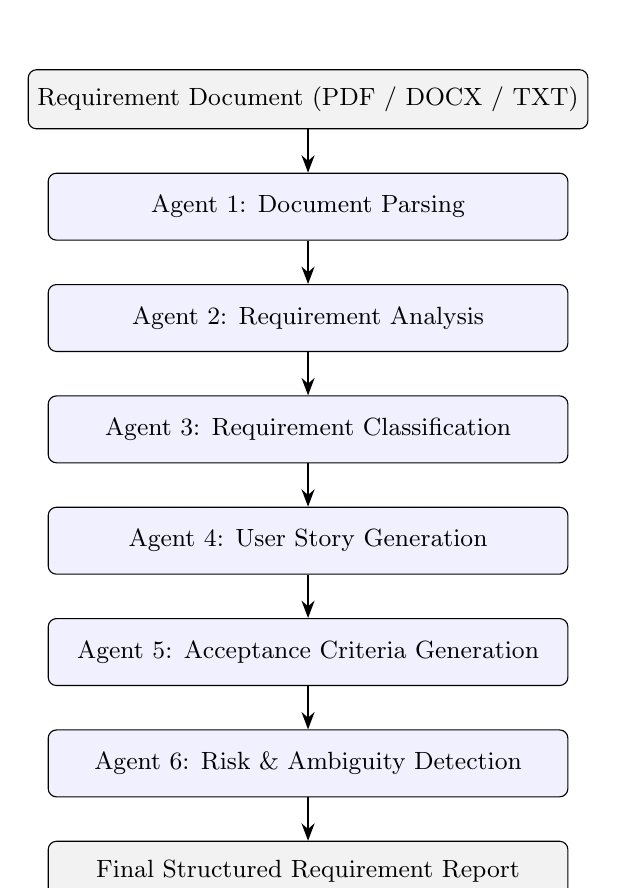
\begin{tikzpicture}[
  node distance=0.55cm and 0.9cm,
  every node/.style={font=\small},
  box/.style={draw, rounded corners=3pt, fill=blue!6, minimum width=6.6cm, minimum height=0.85cm, align=center},
  io/.style={draw, rounded corners=3pt, fill=gray!10, minimum width=6.6cm, minimum height=0.75cm, align=center},
  arr/.style={-{Stealth[length=2.2mm]}, thick}
]
\node[io] (doc) {Requirement Document (PDF / DOCX / TXT)};
\node[box, below=of doc] (a1) {Agent 1: Document Parsing};
\node[box, below=of a1] (a2) {Agent 2: Requirement Analysis};
\node[box, below=of a2] (a3) {Agent 3: Requirement Classification};
\node[box, below=of a3] (a4) {Agent 4: User Story Generation};
\node[box, below=of a4] (a5) {Agent 5: Acceptance Criteria Generation};
\node[box, below=of a5] (a6) {Agent 6: Risk \& Ambiguity Detection};
\node[io, below=of a6] (report) {Final Structured Requirement Report};

\draw[arr] (doc) -- (a1);
\draw[arr] (a1) -- (a2);
\draw[arr] (a2) -- (a3);
\draw[arr] (a3) -- (a4);
\draw[arr] (a4) -- (a5);
\draw[arr] (a5) -- (a6);
\draw[arr] (a6) -- (report);
\end{tikzpicture}
\caption{LangGraph pipeline architecture of the Agentic Requirement Analyzer.}
\label{fig:architecture}
\end{figure}

\section{Shared Pipeline State}
Every agent communicates through a single \texttt{PipelineState}
structure rather than passing ad-hoc arguments between functions. This
was one of the first design decisions made in the project, since it keeps
every agent independently testable.

\begin{lstlisting}[language=Python]
class PipelineState(TypedDict):
    raw_text: str
    filename: str
    actors: list[str]
    features: list[str]
    constraints: list[str]
    functional_requirements: list[str]
    non_functional_requirements: list[str]
    user_stories: list[dict]          # {feature, story, priority}
    acceptance_criteria: list[dict]   # {story_ref, given, when, then}
    risks: list[dict]                 # {requirement, reason, suggestion}
    ambiguities: list[dict]           # {requirement, reason, suggestion}
    errors: list[str]
\end{lstlisting}

\section{Agent Responsibilities}
\begin{longtable}{|p{3.3cm}|p{9.8cm}|}
\caption{Agent Responsibilities in the Pipeline}\\
\hline
\textbf{Agent} & \textbf{Responsibility} \\
\hline
Document Parsing & Detects the uploaded file type and extracts clean text, joining broken lines and stripping whitespace left over from PDF extraction. \\
\hline
Requirement Analysis & Reads the parsed text and identifies actors, system features and constraints. \\
\hline
Requirement Classification & Splits identified requirements into functional and non-functional categories. \\
\hline
User Story Generation & Converts each functional requirement into an Agile user story with a priority level. \\
\hline
Acceptance Criteria Generation & Produces Given/When/Then acceptance criteria for every generated user story. \\
\hline
Risk \& Ambiguity Detection & Embeds each requirement, compares it against a seed corpus of known-vague phrases using FAISS, and asks the LLM to confirm the issue and suggest a concrete fix. \\
\hline
\end{longtable}
\FloatBarrier

% ==================== CHAPTER 4 ====================
\chapter{IMPLEMENTATION}

\section{Document Parsing Agent}
The parsing agent detects the file type from the upload's extension and
routes it to \texttt{pypdf} for PDF files or \texttt{python-docx} for DOCX
files, falling back to a direct read for plain text. Broken lines and
extra whitespace left over from PDF text extraction are cleaned before the
text is passed further down the pipeline.

\section{Requirement Analysis and Classification Agents}
Both agents prompt the Groq-hosted LLM to return \textbf{only valid JSON},
using a one-shot example inside the prompt to anchor the output format.
Each call is wrapped in a retry-once-then-fall-back pattern: if the model
returns malformed JSON, the agent retries a single time and, on repeated
failure, returns empty lists rather than raising an exception. This keeps
a single bad or unusual requirement document from crashing the whole
pipeline mid-run.

\section{User Story and Acceptance Criteria Agents}
For every functional requirement, the User Story agent generates an Agile
story in the ``As a / I want / So that'' format along with an inferred
priority. The Acceptance Criteria agent then takes each generated story
and produces Given/When/Then criteria, using the same retry/fallback
pattern as the earlier agents.

\section{Risk and Ambiguity Detection Agent}
This agent works differently from the others. A small seed corpus of
known-vague phrases (for example ``quickly'', ``user-friendly'', ``as
needed'') is embedded using a Sentence-Transformers model at module load
time and indexed with FAISS. For every requirement, the agent embeds the
requirement text and searches the index for the closest known-vague
phrases. If the similarity is above a threshold, the requirement and the
matched phrase are passed to the LLM together, which confirms the issue
and proposes a concrete rewording -- for example, replacing ``the system
should respond quickly'' with a specific response-time target. In the
current implementation, this agent primarily populates the ambiguities
section; the risks list is reserved for future extension.

\section{Report Assembly}
The final node in the graph combines the outputs of all six agents into
one structured report containing an executive summary, functional and
non-functional requirements, user stories, acceptance criteria, risks,
ambiguous requirements, and suggestions for improvement. Each completed
run is stored in SQLite so it can be revisited from the frontend's history
view.

\section{Frontend}
The React and Tailwind frontend currently provides a file upload form, a
simple step indicator showing the pipeline state, and a results view that
renders the final report in readable sections rather than raw JSON.
Figure~\ref{fig:uploadui} shows the upload interface.

\section{API Endpoints}
The backend exposes the following endpoints for the frontend and manual
testing:

\begin{table}[H]
\centering
\caption{Backend API Endpoints}
\label{tab:api}
\begin{tabularx}{\textwidth}{|p{3.2cm}|X|}
\hline
\textbf{Endpoint} & \textbf{Purpose} \\
\hline
\texttt{GET /health} & Basic health check used to confirm the backend is running. \\
\hline
\texttt{POST /upload} & Accepts a PDF, DOCX or TXT file and stores it under \texttt{uploads/}. \\
\hline
\texttt{POST /analyze/step1} & Runs parsing, analysis and classification only. \\
\hline
\texttt{POST /analyze} & Runs the full pipeline and saves the report in SQLite. \\
\hline
\texttt{GET /runs} & Returns the saved run history. \\
\hline
\texttt{GET /runs/\{run\_id\}} & Returns one stored analysis result by ID. \\
\hline
\end{tabularx}
\end{table}
\FloatBarrier

\begin{figure}[H]
\centering
\includegraphics[width=0.85\textwidth]{assets/upload_ui.png}
\caption{Document upload interface of the Agentic Requirement Analyzer frontend.}
\label{fig:uploadui}
\end{figure}
\FloatBarrier

% ==================== CHAPTER 5 ====================
\chapter{RESULTS AND TESTING}

\section{Testing Approach}
The completed pipeline was tested against sample requirement documents
from three different domains -- e-commerce, healthcare, and HR -- each
written with a deliberate mix of clear and vague requirements so that the
Risk \& Ambiguity agent had something meaningful to flag. Each document
was run through the full pipeline end to end via the \texttt{/analyze}
API endpoint, and the output of every agent was manually reviewed for
correctness before being considered complete.

\section{Sample Output}
Figure~\ref{fig:sampleoutput} shows the pipeline's JSON response for a
sample requirement document, and Figure~\ref{fig:reportview} shows the
same result rendered in the frontend's report view.

\begin{figure}[H]
\centering
\includegraphics[width=0.9\textwidth]{assets/sample_json.png}
\caption{Sample \texttt{/analyze} API response for a test requirement document.}
\label{fig:sampleoutput}
\end{figure}

\begin{figure}[H]
\centering
\includegraphics[width=0.9\textwidth]{assets/report_output.png}
\caption{Final structured report rendered in the frontend, showing requirements, user stories, acceptance criteria and flagged risks.}
\label{fig:reportview}
\end{figure}

\section{Observations}
Across the three sample documents, the Requirement Analysis and
Classification agents consistently separated functional from
non-functional requirements correctly. The Risk \& Ambiguity agent
reliably caught intentionally vague phrasing (for example, unqualified
words like ``fast'' or ``secure'') and proposed specific, measurable
replacements. The main source of variation was in how granular the
generated user stories were for very broad requirements, which was
addressed by refining the prompt to ask for one story per distinct
feature rather than per sentence.

\section{Project Repository}
The complete source code is available on GitHub, as shown in
Figure~\ref{fig:githubrepo}.

\begin{figure}[H]
\centering
\includegraphics[width=0.9\textwidth]{assets/github_repo.png}
\caption{Agentic Requirement Analyzer repository on GitHub.}
\label{fig:githubrepo}
\end{figure}
\FloatBarrier

% ==================== CHAPTER 6 ====================
\chapter{CONCLUSION AND FUTURE SCOPE}

\section{Conclusion}
This internship at \company\ gave me hands-on experience building an
agentic AI system end to end, from choosing an orchestration framework
through to a working frontend. Implementing each of the six agents
individually, rather than as one large prompt, made the system easier to
debug, test and reason about, and reflected how a real business analyst's
workflow is actually broken into discrete steps. Working with LangGraph,
FastAPI, and FAISS-based similarity search over the four weeks
strengthened my understanding of both agentic AI system design and
practical backend engineering.

\section{Future Scope}
Beyond the scope of this internship, the system could be extended with
Jira or Azure DevOps integration to push generated user stories directly
into a sprint board, UML and database schema generation from the same
parsed requirements, multi-language requirement support, and an
effort-estimation agent that assigns story points based on similar past
requirements.

% ==================== REFERENCES ====================
\chapter*{REFERENCES}
\addcontentsline{toc}{chapter}{References}
\begin{enumerate}[leftmargin=*,label={[\arabic*]}]
\item Agentic Requirement Analyzer Code Repository,\\ \url{https://github.com/haripatel07/agentic-requirement-analyzer}
\item LangChain AI, LangGraph Documentation, \url{https://langchain-ai.github.io/langgraph/}
\item FastAPI Documentation, \url{https://fastapi.tiangolo.com/}
\item Groq API Documentation, \url{https://console.groq.com/docs}
\item pypdf Documentation, \url{https://pypdf.readthedocs.io/}
\item python-docx Documentation, \url{https://python-docx.readthedocs.io/}
\item Reimers, N., \& Gurevych, I., Sentence-BERT: Sentence Embeddings using Siamese BERT-Networks, EMNLP 2019.
\item Johnson, J., Douze, M., \& J\'egou, H., Billion-scale similarity search with GPUs, IEEE Transactions on Big Data, 2019.
\item Cohn, M., User Stories Applied: For Agile Software Development, Addison-Wesley, 2004.
\item Wiegers, K., \& Beatty, J., Software Requirements, Microsoft Press, 2013.
\end{enumerate}

\end{document}